\documentclass[10pt]{article}
\usepackage[a4paper,landscape,margin=12mm]{geometry}
\usepackage[T1]{fontenc}\usepackage{mathpazo,amsmath,amssymb,tikz,booktabs,array}
\usetikzlibrary{arrows.meta,positioning,calc}
\usepackage[hidelinks]{hyperref}
\setlength{\parindent}{0pt}\setlength{\parskip}{4pt}
\pagestyle{empty}
\tikzset{result/.style={draw=blue!55!black,fill=blue!4,rounded corners=3pt,align=center,text width=4.35cm,minimum height=1.25cm,font=\small},
module/.style={result,draw=teal!65!black,fill=teal!5},
assumption/.style={result,draw=gray!70,fill=gray!7},
extension/.style={result,draw=orange!75!black,fill=orange!7},
edge/.style={-{Stealth[length=2mm]},line width=.75pt,draw=blue!55!black},
reuse/.style={edge,dashed,draw=orange!75!black}}
\begin{document}
{\LARGE\bfseries CCSGD: theorem dependency graph}\hfill Source snapshot: 11 October 2026\par
Solid arrows: proof dependencies. Dashed arrows: conditional reuse. Assumption groups label the contract; each result's full assumptions and source coordinates are in the JSON. Transitive result edges are suppressed here.\par
\begin{center}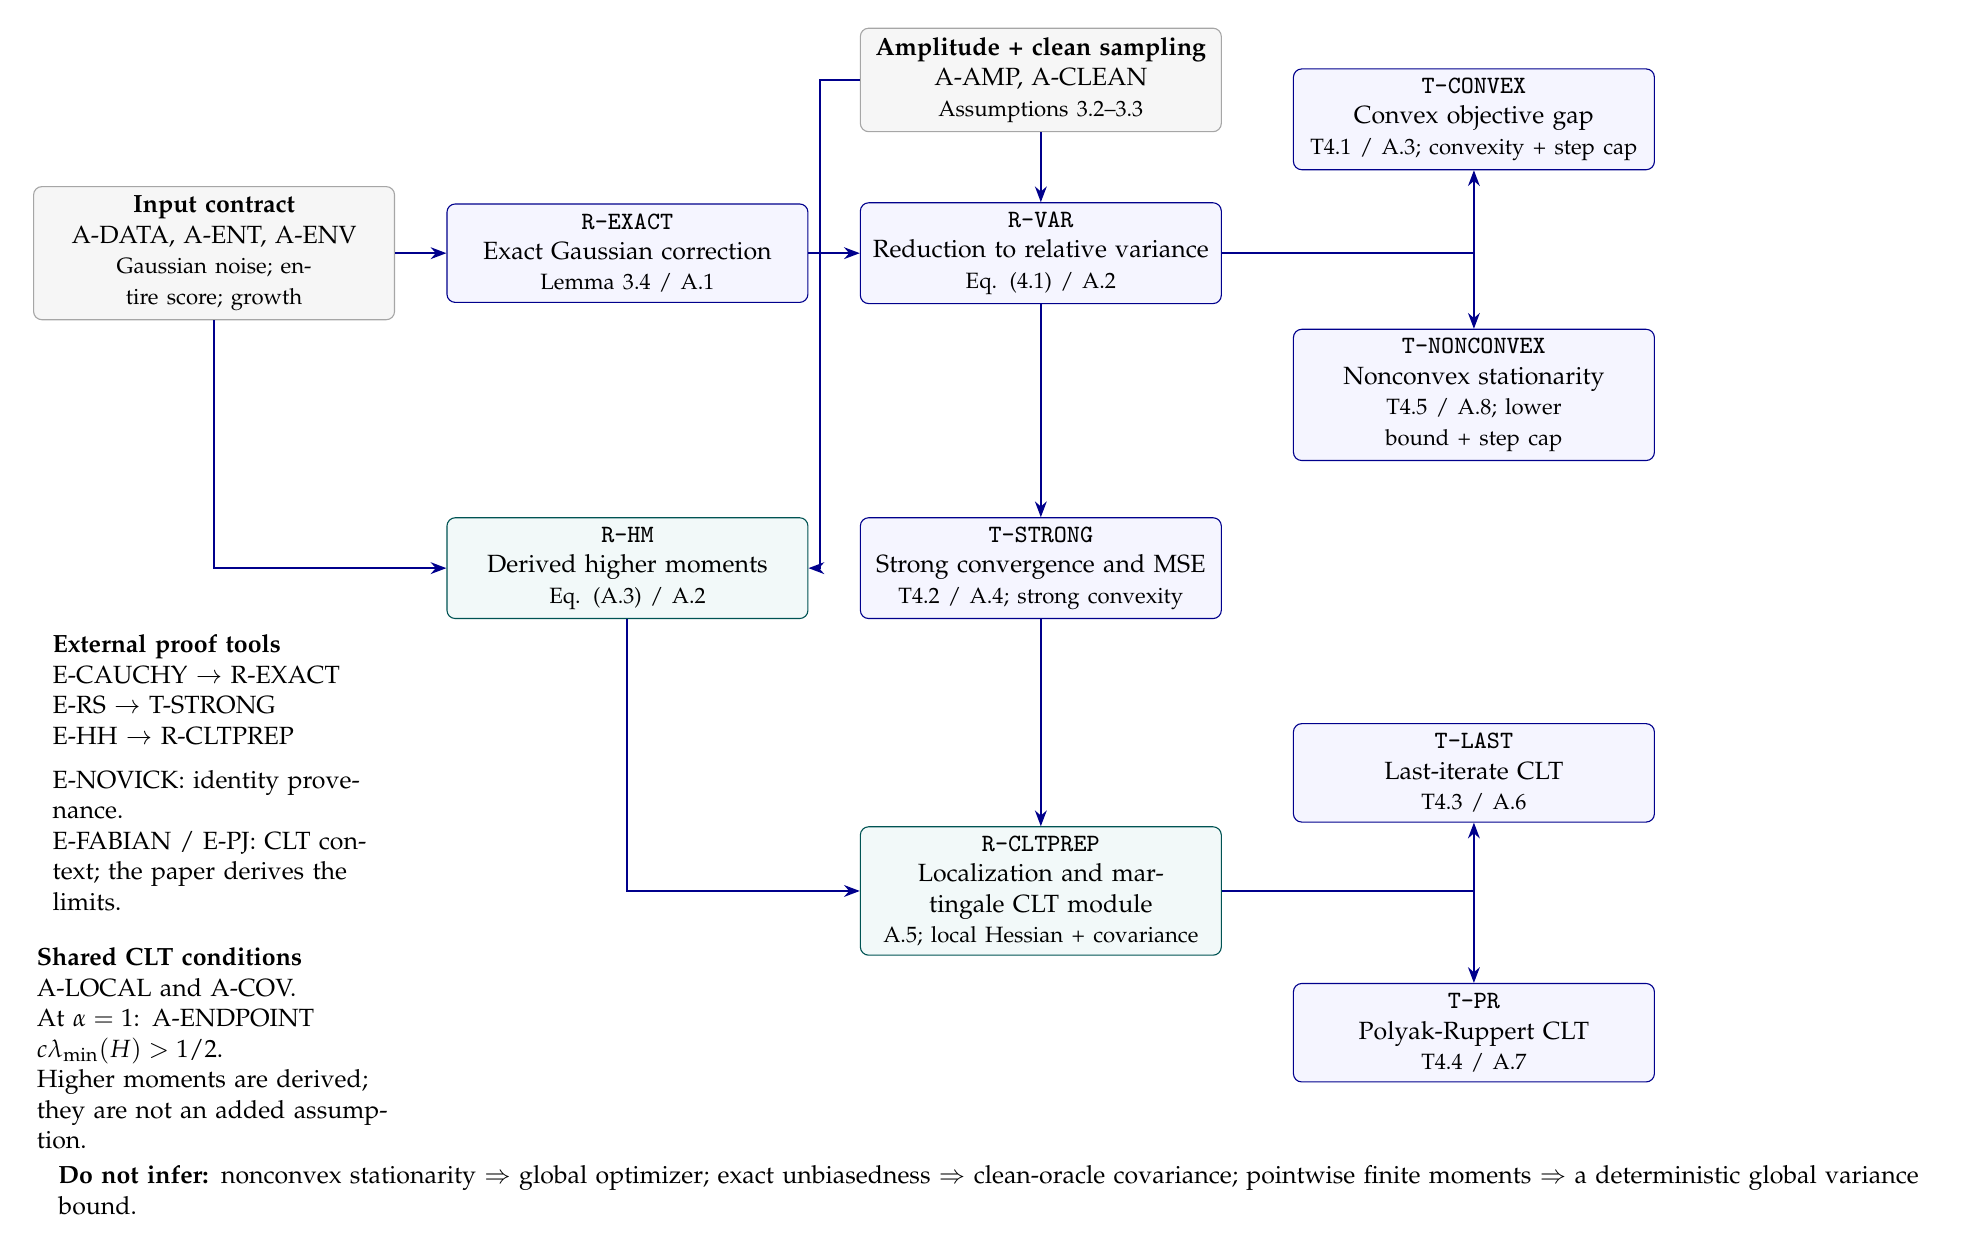
\begin{tikzpicture}[x=1cm,y=1cm]
\node[assumption] (INPUT) at (2.1,11.8) {\textbf{Input contract}\\A-DATA, A-ENT, A-ENV\\{\footnotesize Gaussian noise; entire score; growth}};
\node[assumption] (AMP) at (12.6,14.0) {\textbf{Amplitude + clean sampling}\\A-AMP, A-CLEAN\\{\footnotesize Assumptions 3.2--3.3}};
\node[result] (R-EXACT) at (7.35,11.8) {\textbf{\texttt{R-EXACT}}\\Exact Gaussian correction\\{\footnotesize Lemma 3.4 / A.1}};
\node[result] (R-VAR) at (12.6,11.8) {\textbf{\texttt{R-VAR}}\\Reduction to relative variance\\{\footnotesize Eq. (4.1) / A.2}};
\node[module] (R-HM) at (7.35,7.8) {\textbf{\texttt{R-HM}}\\Derived higher moments\\{\footnotesize Eq. (A.3) / A.2}};
\node[result] (T-STRONG) at (12.6,7.8) {\textbf{\texttt{T-STRONG}}\\Strong convergence and MSE\\{\footnotesize T4.2 / A.4; strong convexity}};
\node[result] (T-CONVEX) at (18.1,13.5) {\textbf{\texttt{T-CONVEX}}\\Convex objective gap\\{\footnotesize T4.1 / A.3; convexity + step cap}};
\node[result] (T-NONCONVEX) at (18.1,10) {\textbf{\texttt{T-NONCONVEX}}\\Nonconvex stationarity\\{\footnotesize T4.5 / A.8; lower bound + step cap}};
\node[module] (R-CLTPREP) at (12.6,3.7) {\textbf{\texttt{R-CLTPREP}}\\Localization and martingale CLT module\\{\footnotesize A.5; local Hessian + covariance}};
\node[result] (T-LAST) at (18.1,5.2) {\textbf{\texttt{T-LAST}}\\Last-iterate CLT\\{\footnotesize T4.3 / A.6}};
\node[result] (T-PR) at (18.1,1.9) {\textbf{\texttt{T-PR}}\\Polyak-Ruppert CLT\\{\footnotesize T4.4 / A.7}};
\draw[edge] (INPUT) -- (R-EXACT);
\draw[edge] (R-EXACT) -- (R-VAR);
\draw[edge] (AMP) -- (R-VAR);
\draw[edge] (INPUT) |- (R-HM);
\draw[edge] (AMP.west) -- (9.8,14.0) -- (9.8,7.8) -- (R-HM.east);
\draw[edge] (R-VAR) -| (T-CONVEX);
\draw[edge] (R-VAR) -| (T-NONCONVEX);
\draw[edge] (R-VAR) -- (T-STRONG);
\draw[edge] (T-STRONG) -- (R-CLTPREP);
\draw[edge] (R-HM) |- (R-CLTPREP);
\draw[edge] (R-CLTPREP) -| (T-LAST);
\draw[edge] (R-CLTPREP) -| (T-PR);
\node[align=left,text width=4.1cm,font=\small] at (2.1,5.2) {\textbf{External proof tools}\\E-CAUCHY $\to$ R-EXACT\\E-RS $\to$ T-STRONG\\E-HH $\to$ R-CLTPREP\\[5pt]E-NOVICK: identity provenance.\\E-FABIAN / E-PJ: CLT context; the paper derives the limits.};
\node[align=left,text width=4.5cm,font=\small] at (2.1,1.7) {\textbf{Shared CLT conditions}\\A-LOCAL and A-COV.\\At $\alpha=1$: A-ENDPOINT\\$c\lambda_{\min}(H)>1/2$.\\Higher moments are derived;\\they are not an added assumption.};
\node[align=left,text width=24cm,font=\small,anchor=west] at (0,-.1) {\textbf{Do not infer:} nonconvex stationarity $\Rightarrow$ global optimizer; exact unbiasedness $\Rightarrow$ clean-oracle covariance; pointwise finite moments $\Rightarrow$ a deterministic global variance bound.};
\end{tikzpicture}\end{center}
\clearpage
{\LARGE\bfseries Extensions, proof locations, and external status}\par
\begin{center}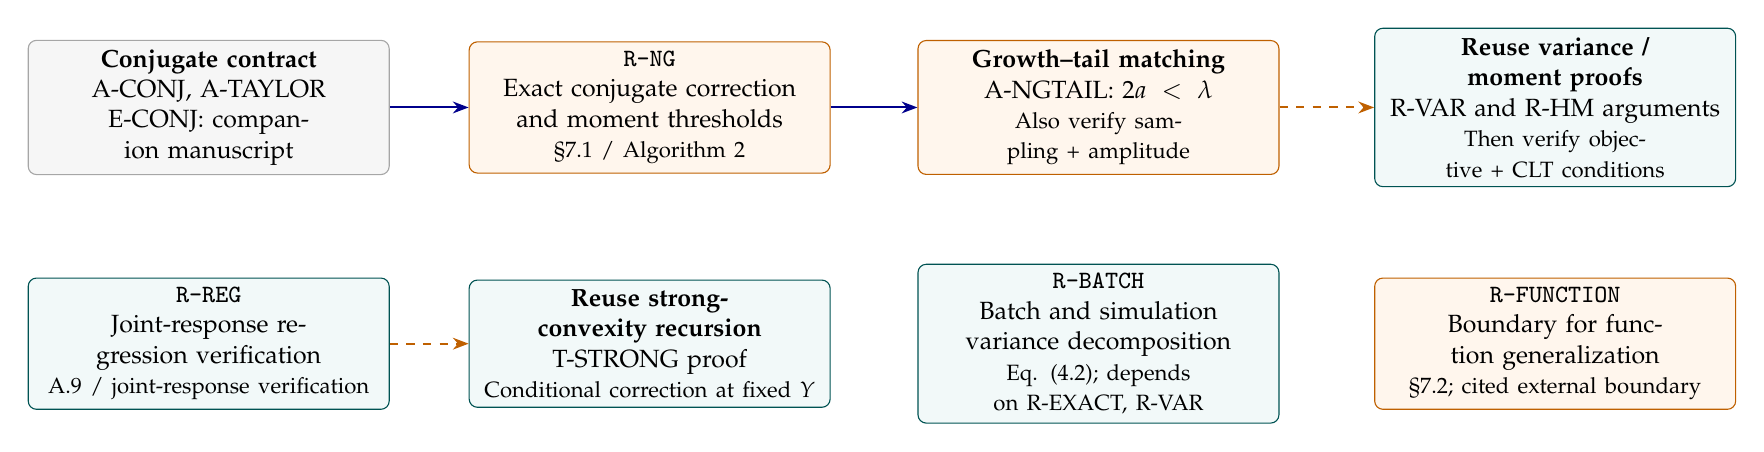
\begin{tikzpicture}[x=1cm,y=1cm]
\node[assumption] (CONJ) at (2.2,3.7) {\textbf{Conjugate contract}\\A-CONJ, A-TAYLOR\\E-CONJ: companion manuscript};
\node[extension] (R-NG) at (7.8,3.7) {\textbf{\texttt{R-NG}}\\Exact conjugate correction and moment thresholds\\{\footnotesize \S7.1 / Algorithm 2}};
\node[extension] (NGMOM) at (13.5,3.7) {\textbf{Growth--tail matching}\\A-NGTAIL: $2a<\lambda$\\{\footnotesize Also verify sampling + amplitude}};
\node[module] (REUSE) at (19.3,3.7) {\textbf{Reuse variance / moment proofs}\\R-VAR and R-HM arguments\\{\footnotesize Then verify objective + CLT conditions}};
\draw[edge] (CONJ) -- (R-NG);
\draw[edge] (R-NG) -- (NGMOM);
\draw[reuse] (NGMOM) -- (REUSE);
\node[module] (R-REG) at (2.2,0.7) {\textbf{\texttt{R-REG}}\\Joint-response regression verification\\{\footnotesize A.9 / joint-response verification}};
\node[module] (REGREUSE) at (7.8,.7) {\textbf{Reuse strong-convexity recursion}\\T-STRONG proof\\{\footnotesize Conditional correction at fixed $Y$}};
\draw[reuse] (R-REG) -- (REGREUSE);
\node[module] (R-BATCH) at (13.5,0.7) {\textbf{\texttt{R-BATCH}}\\Batch and simulation variance decomposition\\{\footnotesize Eq. (4.2); depends on R-EXACT, R-VAR}};
\node[extension] (R-FUNCTION) at (19.3,0.7) {\textbf{\texttt{R-FUNCTION}}\\Boundary for function generalization\\{\footnotesize \S7.2; cited external boundary}};
\end{tikzpicture}\end{center}
\vspace{2mm}
\begin{minipage}[t]{.49\linewidth}
\textbf{Stable result registry}\par\small
\begin{tabular}{@{}p{.22\linewidth}p{.32\linewidth}p{.35\linewidth}@{}}\toprule
ID & Paper location & Proof location \\\midrule
\texttt{R-EXACT} & Lemma 3.4 & A.1 \\
\texttt{R-VAR} & Eq. (4.1) & A.2 \\
\texttt{R-HM} & Eq. (A.3) & A.2 \\
\texttt{R-BATCH} & Eq. (4.2) & Before T4.1 \\
\texttt{T-CONVEX} & Theorem 4.1 & A.3 \\
\texttt{T-STRONG} & Theorem 4.2 & A.4 \\
\texttt{R-CLTPREP} & Appendix A.5 & A.5 \\
\texttt{T-LAST} & Theorem 4.3 & A.5--A.6 \\
\texttt{T-PR} & Theorem 4.4 & A.5, A.7 \\
\texttt{T-NONCONVEX} & Theorem 4.5 & A.8 \\
\texttt{R-REG} & Appendix A.9 & A.9 \\
\texttt{R-NG} & Section 7.1 & Section 7.1 \\
\texttt{R-FUNCTION} & Section 7.2 & External result \\
\bottomrule\end{tabular}\par
R-NG is a conditional extension discussed with a derivation, not a newly numbered non-Gaussian convergence theorem. R-FUNCTION records an external scope restriction.
\end{minipage}\hfill
\begin{minipage}[t]{.49\linewidth}
\textbf{External dependency status}\par\small
\begin{tabular}{@{}p{.23\linewidth}p{.67\linewidth}@{}}\toprule
ID & Status in this repository \\\midrule
E-CAUCHY & Standard complex-analysis tool; not reproved. \\
E-NOVICK & Cited historical identity; correction reproved internally. \\
E-RS & Cited convergence theorem; recursion verified internally. \\
E-HH & Cited martingale CLT; its conditions checked internally. \\
E-FABIAN & CLT context; product/covariance derivation is internal. \\
E-PJ & Averaging context; both step-size regimes derived internally. \\
E-CONJ & Companion source consulted; not bundled or independently certified. \\
E-STEFANSKI & Cited Gaussian function-class boundary; not reproved. \\
\bottomrule\end{tabular}\par
\textbf{Machine version.} \texttt{theorem\_graph.json} contains every assumption, complete conclusion, direct result dependency, proof file/line/anchor, PDF page, and external status. It is the source for this diagram.\par
\textbf{Review status.} A user-provided 6 Astra review reports no major gaps for \texttt{main(6).pdf}; file-level correspondence with this snapshot is unconfirmed. See \texttt{reviews/6\_astra/}. This graph is not independent certification.
\end{minipage}
\end{document}
